\documentclass[10pt]{beamer}
\usepackage{xeCJK}
\usepackage{graphicx}
\usepackage{booktabs}
\usepackage{listings}
\usepackage{multirow}
\usepackage{mathtools}
\usepackage{pdfpages}
\usepackage{ulem}
\usefonttheme[onlymath]{serif}
\usetheme{metropolis}
\setbeamercolor{footnote mark}{fg=blue}% set footnote color in beamer
\setbeamerfont{footnote}{size=\tiny}
\begin{document}
	\title{线性代数}
	\date{\today}
	\author{huhao}
	\maketitle
	\clearpage
	\begin{frame}
		\frametitle{基础知识}
	
		\begin{itemize}
			\item 线性空间
			\item 基
			\item 线性变换
			\item 矩阵、基变换
		\end{itemize}
	
	\end{frame}
	\begin{frame}
		\frametitle{特征值、特征向量、特征多项式}

		对于矩阵$A$,满足$Av=\lambda v$的$\lambda$是特征值,$v$是特征向量。

		不难发现,当且仅当$\det(A-\lambda I)=0$,$\lambda$是特征向量,不妨称$f(x)=\det(A-x I)$为$A$的特征多项式。
	\end{frame}
	\begin{frame}
		\frametitle{例}
	
		求:

		$$
		\begin{bmatrix}
		&1\\
		&&1\\
		&&&\ddots\\
		&&&&1\\
		a_1&a_2&a_3&\dots&a_n
		\end{bmatrix}
		$$

		的特征多项式。
	
	\end{frame}
	\begin{frame}
		\frametitle{Cayley–Hamilton Theorem}
	
		若$f$是$A$的特征多项式,则$f(A)=0$。

		所以$A^n=(x^n \bmod f)|_{x=A}$。

		综合此页和上一页的内容可以得到常系数齐次线性递推的做法。
	
	\end{frame}
	\begin{frame}
		\frametitle{矩阵对角化}
	
		如果矩阵$A$有$n=\dim A$个线性无关的特征向量$\alpha_1\dots\alpha_n$,那么它在$\alpha$下的矩阵是对角矩阵。

		令$P$为所有线性无关的特征向量(列向量)拼接组成的矩阵,则:

		$$
		D=P^{-1}AP
		$$

		为对角矩阵。
	
	\end{frame}
	\begin{frame}
		\frametitle{例}
		
		对角化:
		
		$$
		\begin{bmatrix}
			1&2&3\\
			4&5&6\\
			7&8&9
		\end{bmatrix}
		$$
	\end{frame}
	\begin{frame}
		\frametitle{}
		
		\begin{center}
			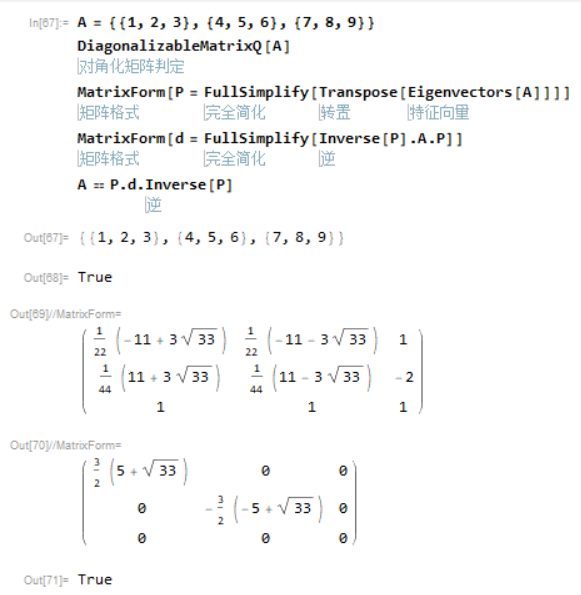
\includegraphics[width=0.7\textwidth]{1.PNG}
		\end{center}
	
	\end{frame}
	\begin{frame}
		\frametitle{Jordan型}
	
		不一定所有矩阵都可以找到$n$个线性无关的特征向量。

		\begin{center}
			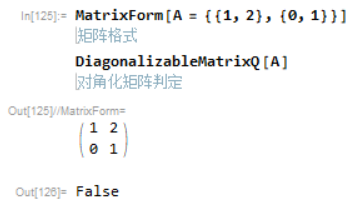
\includegraphics[width=0.5\textwidth]{2.PNG}
		\end{center}

		但是,如果将$(A-\lambda I)^{\dim A} v=0$的$v$称为广义特征向量,那么一定会有$\dim A$个线性无关广义特征向量。
	
	\end{frame}
	\begin{frame}
		\frametitle{}
	
		考虑若干个$v_{1,1}\dots v_{1,m_1}\dots v_{k,1}\dots v_{k,m_k}$是$n$个线性无关的广义特征向量,且:
		
		$$
		(A-\lambda_i I)v_{i,j}=v_{i,j+1}
		$$

		那么$A$在这组基下就是:
		$$
		\begin{bmatrix}
			A_1\\
			&A_2\\
			&&\ddots\\
			&&&A_k
		\end{bmatrix}
		$$
		
		且$A_i$是大小为$m_i$,对角线和对角线上面一格为$1$其它为$0$的矩阵。

		这样子的$A$可以很方便的计算幂。
	\end{frame}
	\begin{frame}
		\frametitle{例}
	
		计算
		
		$$
		\begin{bmatrix}
			&1\\
			&&1\\
			-1&-3&-3
		\end{bmatrix}^n
		$$
	
	\end{frame}
	\begin{frame}
		\frametitle{}
	
		\begin{center}
			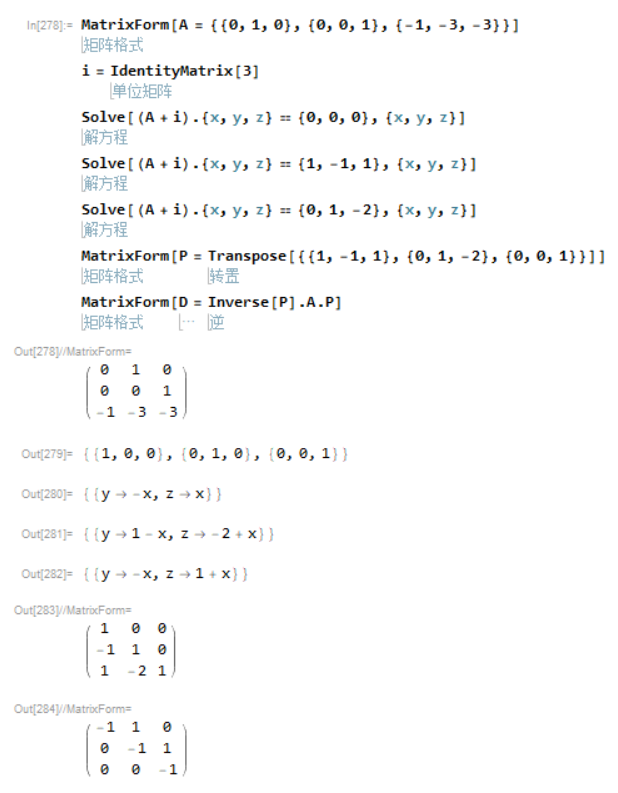
\includegraphics[width=0.66\textwidth]{3.PNG}
		\end{center}	
	
	\end{frame}
	\begin{frame}
		\frametitle{}
	
		当然也可以用mathematica内置的。
	
		\begin{center}
			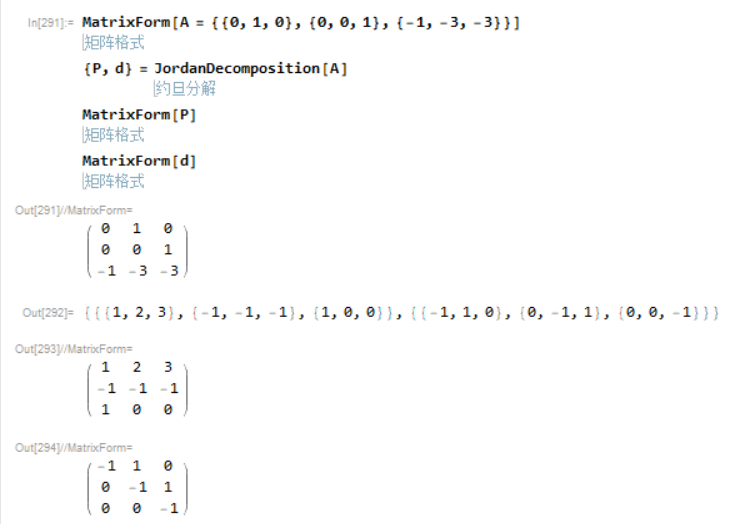
\includegraphics[width=\textwidth]{4.PNG}
		\end{center}	
	
	\end{frame}	
	\begin{frame}
		\frametitle{}
	
		这个幂是很容易算的

		\begin{center}
			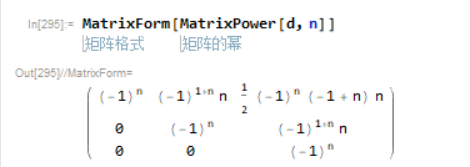
\includegraphics[width=\textwidth]{5.PNG}
		\end{center}	
	
	\end{frame}
	\begin{frame}
		\frametitle{例}
	
		$A$是上三角矩阵,求$A^k$,其中$n$远小于$\log k$。
	
	\end{frame}
	\begin{frame}
		\frametitle{QR分解}
	
		矩阵的QR分解是一个很重要的算法,对于矩阵$A$,要求出正交矩阵$Q$和上三角矩阵$R$使得:

		$$
		A=QR
		$$

		分解方法为对$A$的每一个列向量$a_i$使用Gram–Schmidt过程得到$e_i$,然后:

		$$
		\begin{aligned}
			Q=&[e_i]\\
			R=&[\langle e_i,a_j\rangle]
		\end{aligned}
		$$
	
	\end{frame}
	\begin{frame}
		\frametitle{QR算法}
	
		可以参考:\url{https://pi.math.cornell.edu/~web6140/TopTenAlgorithms/QRalgorithm.html}
		
		若要求$A$的特征值,可以令$A_0=A$,且:$A_i=Q_iR_i,A_{i+1}=R_iQ_i$,则:

		$$
		A_{i+1}=R_iQ_i=Q_i^{-1}Q_iR_iQ_i=Q_i^{-1}A_iQ_i
		$$

		不难发现,$A_{i+1}$和$A_i$相似,有着相同的特征值。

		不断这样计算,直到收敛至上三角矩阵。
	
	\end{frame}
	\begin{frame}
		\frametitle{上海森伯格化}
	
		海森伯格矩阵是只有对角线上方,以及对角线下一个元素非0的矩阵。

		考虑
		
		$$
		A=\begin{bmatrix}
			a&A_1\\A_2&A_3
		\end{bmatrix}
		$$

		那么如果$T_i$是满足$TA_2=e_1$,那么:

		$$
		\begin{bmatrix}
			1\\&T_i
		\end{bmatrix}A\begin{bmatrix}
			1\\&T_i^{-1}
		\end{bmatrix}
		$$

		可以将第$1$列$3\sim$变为$0$,然后一次做第$2\dots $列即可。

		令$\hat T_i=\begin{bmatrix}
			1\\&\ddots\\&&T_i
		\end{bmatrix}$这样可以得到$\hat T=\hat T_{n-2}\dots \hat T_1$满足$\hat TA\hat T^{-1}$是海森伯格矩阵。
	
	\end{frame}
	\begin{frame}
		\frametitle{上海森伯矩阵的QR分解}
	
		考虑相邻两行,对这两行应用旋转变换:

		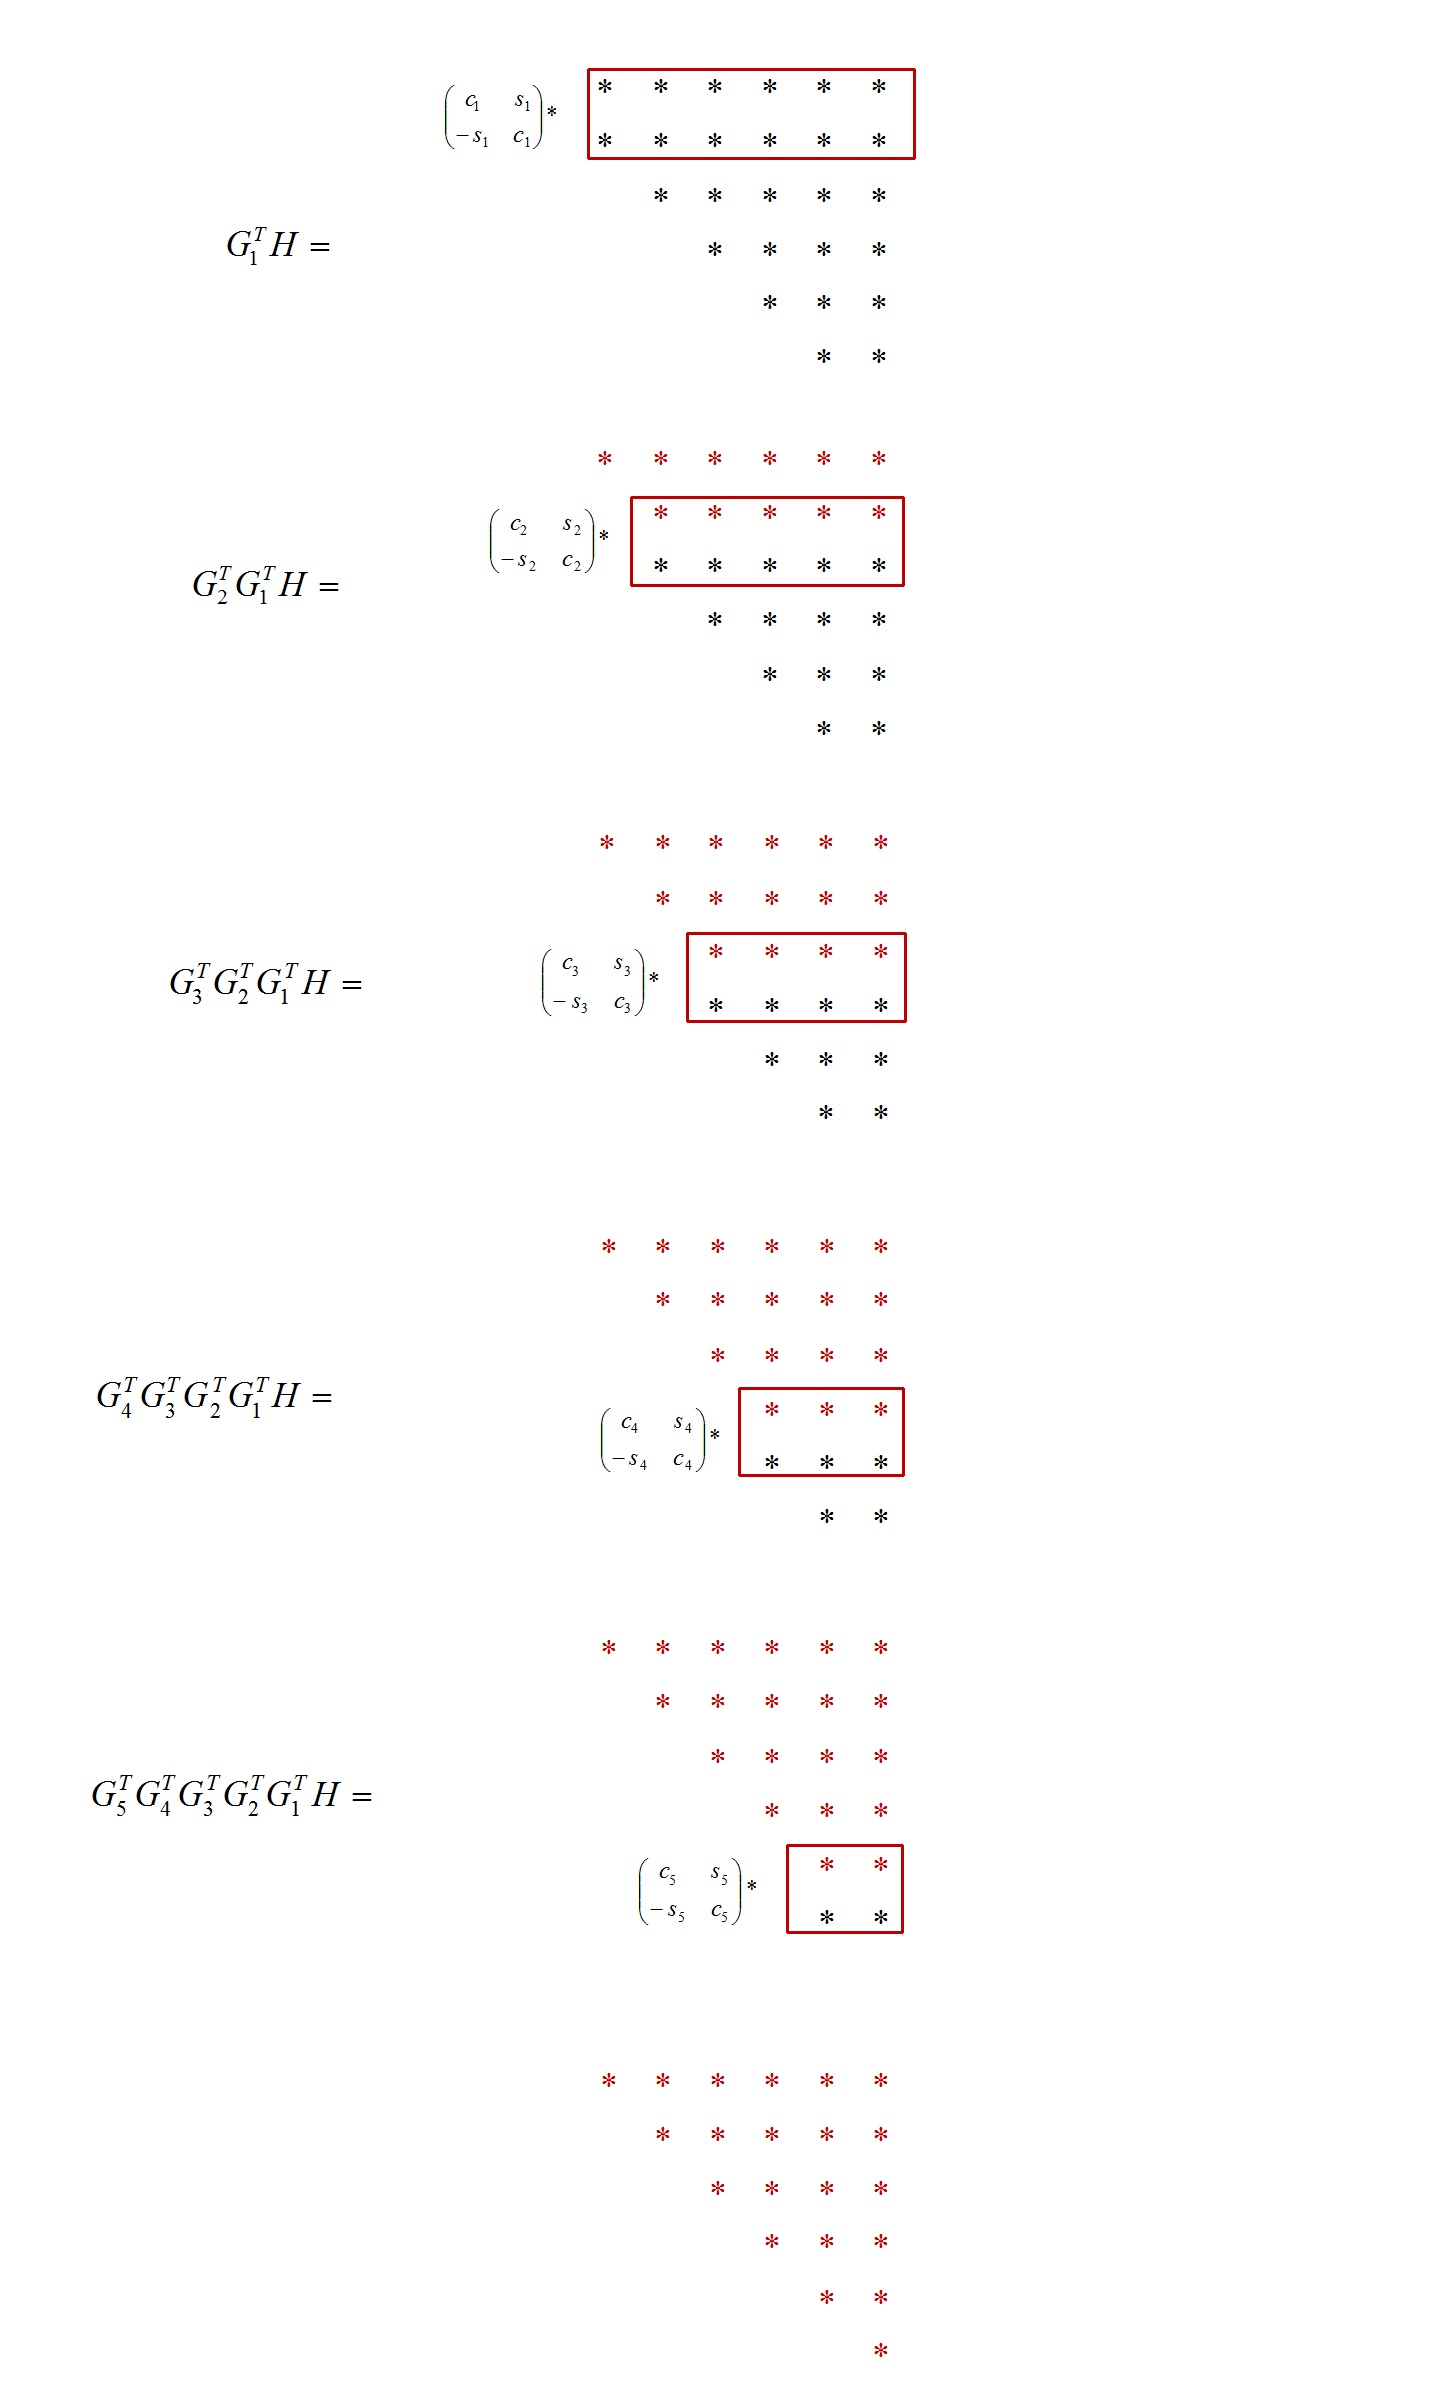
\includegraphics[width=0.7\textwidth]{6.jpg}

	\end{frame}
	\begin{frame}
		\frametitle{}
	
		可以发现,逆回来也是上海森伯矩阵:

		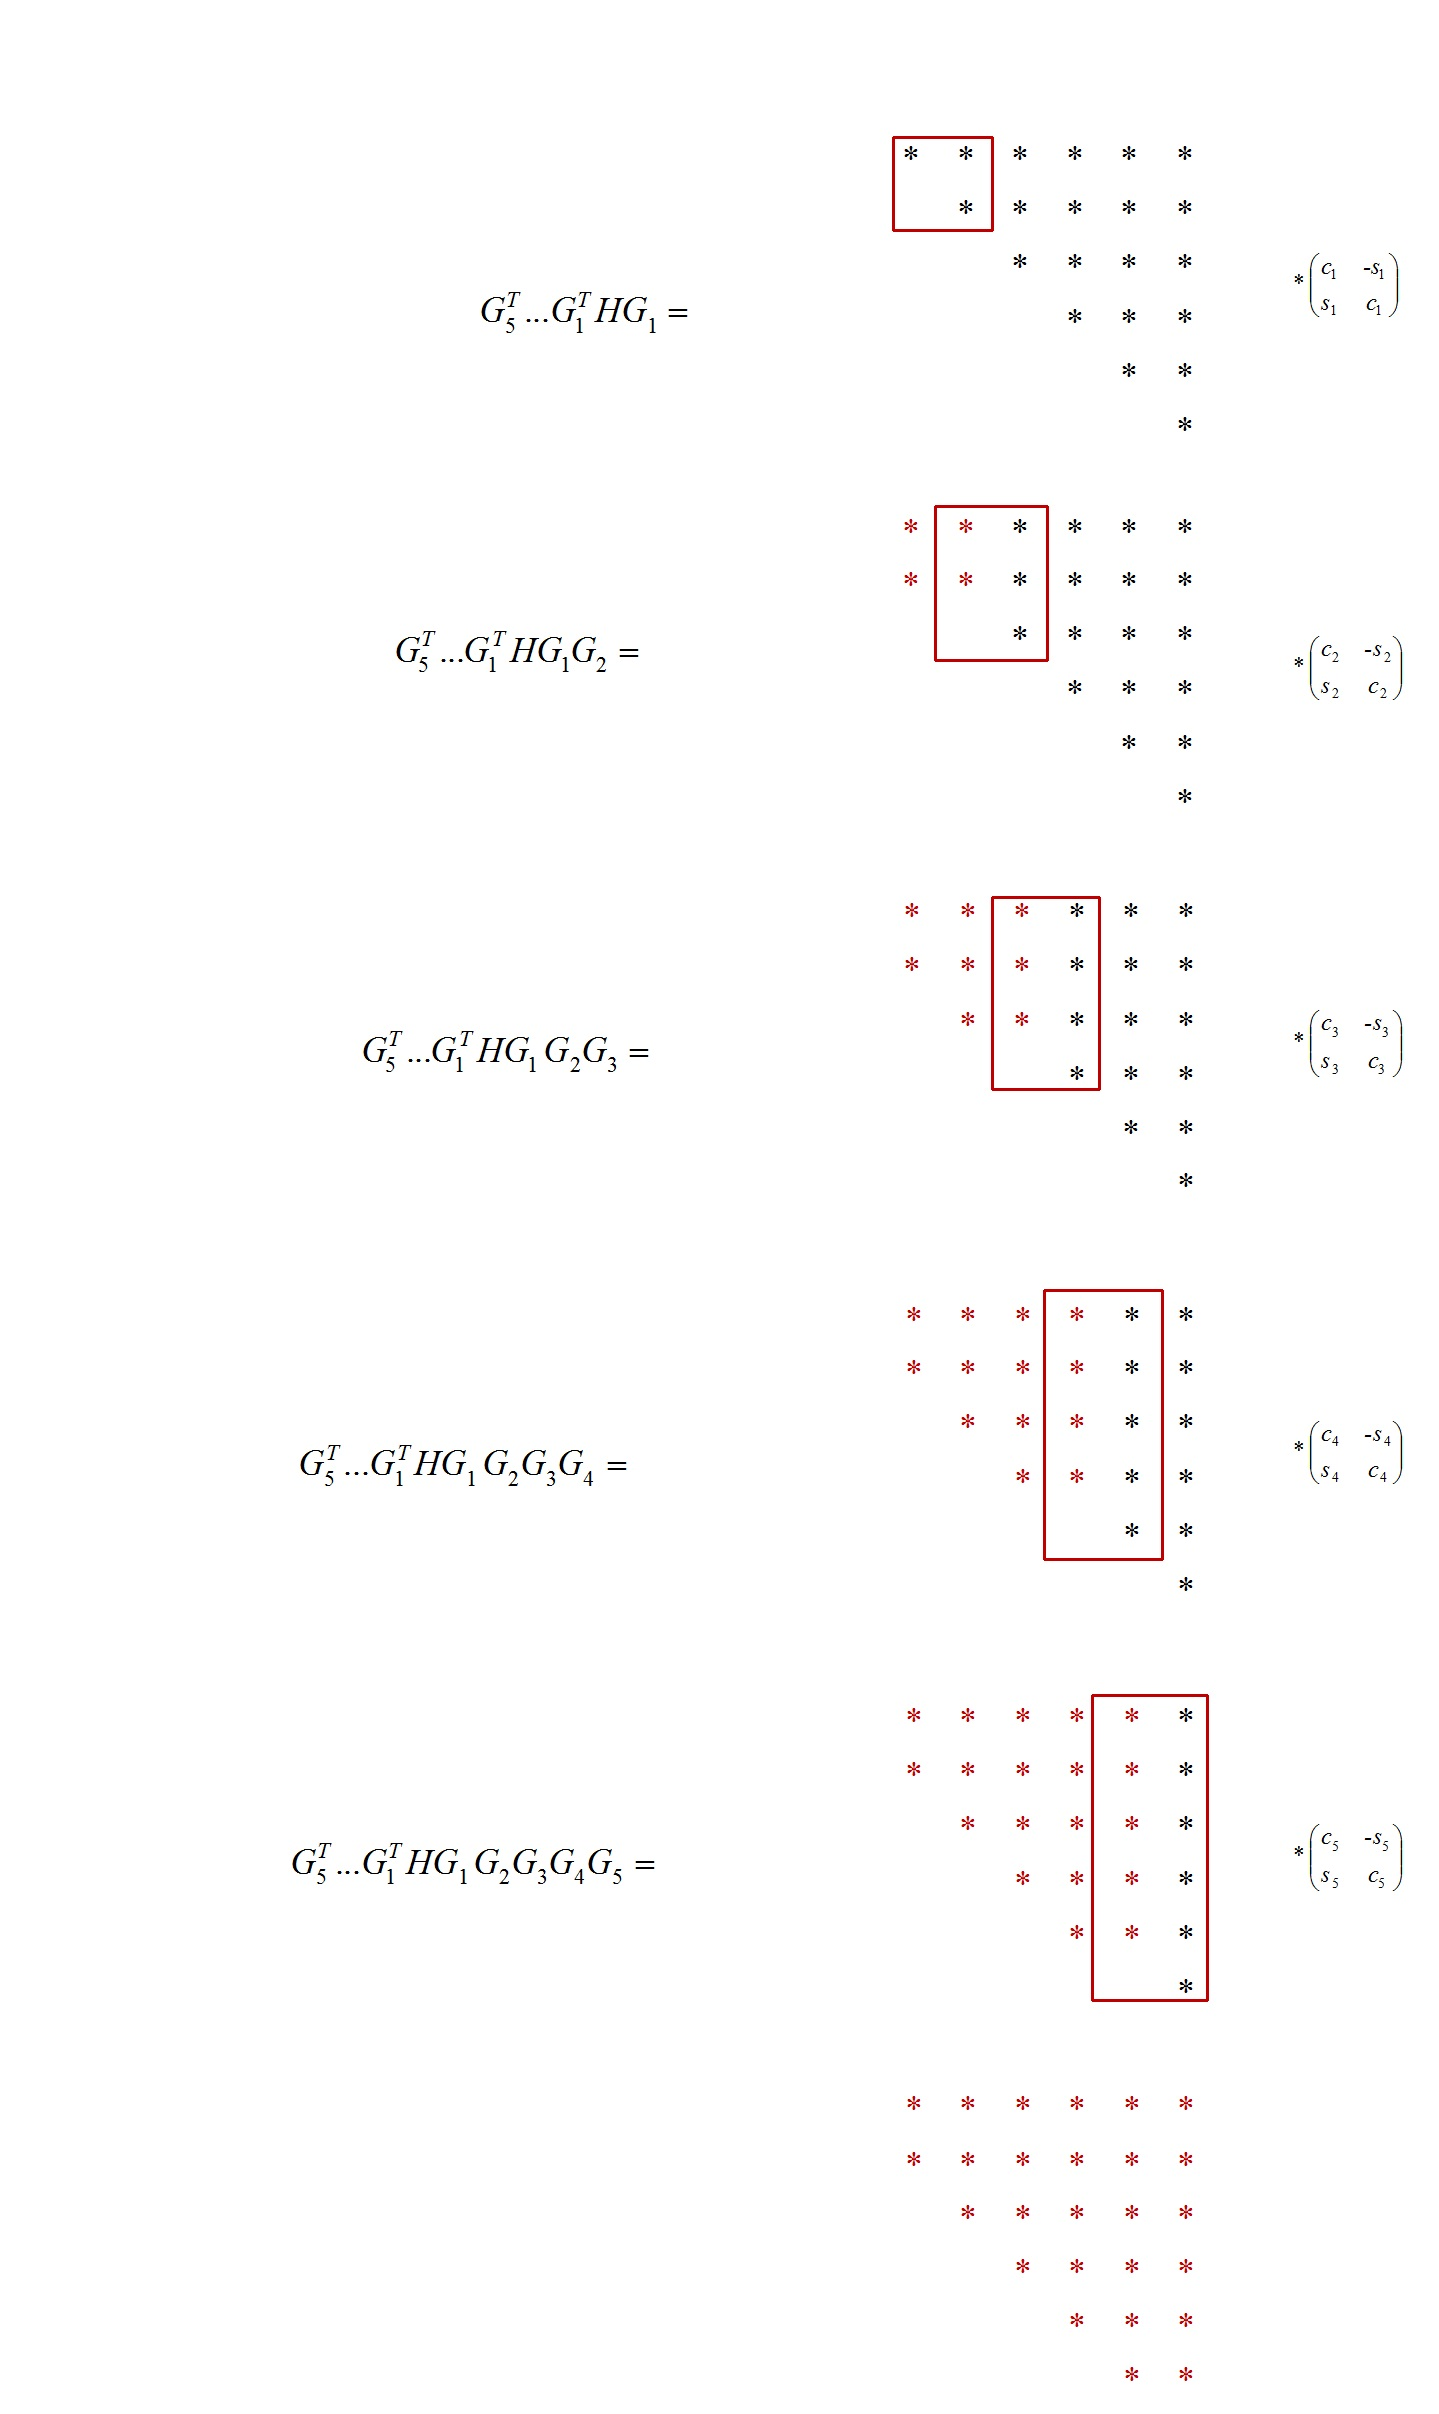
\includegraphics[width=0.7\textwidth]{7.jpg}

	\end{frame}
	\begin{frame}
		\frametitle{平移加速}
	
		一般来说,$A$的特征值间差异越大,QR算法收敛越快。

		不妨令:

		$$
		A_i-\delta I=QR,A_{i+1}=RQ+\delta I
		$$

		那么$A_{i+1}$的特征值和$A_i$的特征值依然是一样的。

		一般来说,$\delta$可以取$A$对角线上的$2\times 2$的方阵的特征值。
	
	\end{frame}
\end{document}